\chapter{Results and Discussions}\label{ch:result_discussion}
This chapter briefly discusses the datasets we used to train and evaluate our model, and the results our proposed algorithm achieved at different experimental setup. As to estimate pose, RGB video frames are required. So, we couldn't evaluate our method to those dataset which only consists of silhouette sequences.


%-------------------------------------------------------------------------
\section{Dataset}
The success of deep learning-based methods greatly depends on the vast amount of labeled train data. Unfortunately, few existing gait databases contain a large number of subjects as well as a variety of covariate factors. Some of the publicly available gait databases are CASIA gait dataset~\cite{Yu_06}, TUM GAID dataset~\cite{Hofmann_14}, OU-ISIR multi-view large population dataset (OU-MVLP)~\cite{Noriko_18} and USF HumanID dataset~\cite{Sarkar_05}. 

In USF HumanID gait dataset, there are $ 122 $ subjects walking outside on two different surfaces of an elliptical path under two different time, viewpoint, clothing, shoes, and carrying conditions. However, not all subjects were filmed under all conditions. TUM GAID dataset is another large dataset for gait recognition which consists of $ 305 $ subjects where each subject has $ 10 $ videos. But this dataset is not suitable for multi-view gait recognition as all the videos were recorded from side view angle. The largest dataset available for gait recognition is OU-ISIR multi-view large population dataset (OU-MVLP). It contains $ 10,307 $ subjects from $ 14 $ view angles ranging from ${{0}^{\circ}-{90}^{\circ}}$, ${{180}^{\circ}-{270}^{\circ}}$. Only two sequences are provided, one for the gallery and the other for the probe. But, this dataset is formatted only as a set of silhouette sequence making it different from our approach.

In this study, we used CASIA (both CASIA A and CASIA B) dataset which is one of the largest multi-view gait databases. CASIA A dataset contains total $ 20 $ subjects walking in an outdoor environment where CASIA B dataset includes total $ 124 $ subjects walking in an indoor environment. In CASIA A gait dataset, each subject walks along a straight line in 3 different view angles lateral (${0^{\circ}}$), oblique (${45^{\circ}}$) and frontal (${90^{\circ}}$). For each viewing angle every subject has four gait sequences of which two of them have same walking direction while the other two have opposite direction. In CASIA B dataset, there are 10 walking sequences of each subject captured from 11 view angles: 6 sequences for normal walking ('nm'), 2 sequences for walking in a coat ('cl') and 2 sequences for walking with bag ('bg') on shoulder. Hence, this dataset separately considered three variations in people walking namely viewing angle, clothing and carrying conditions. The view angle set of the camera is ranging from ${0^{\circ}}$ to ${180^{\circ}}$. Figure~\ref{fig:casia_dataset} illustrates some of the sample video frames of CASIA dataset.


\begin{figure}
	\centering
	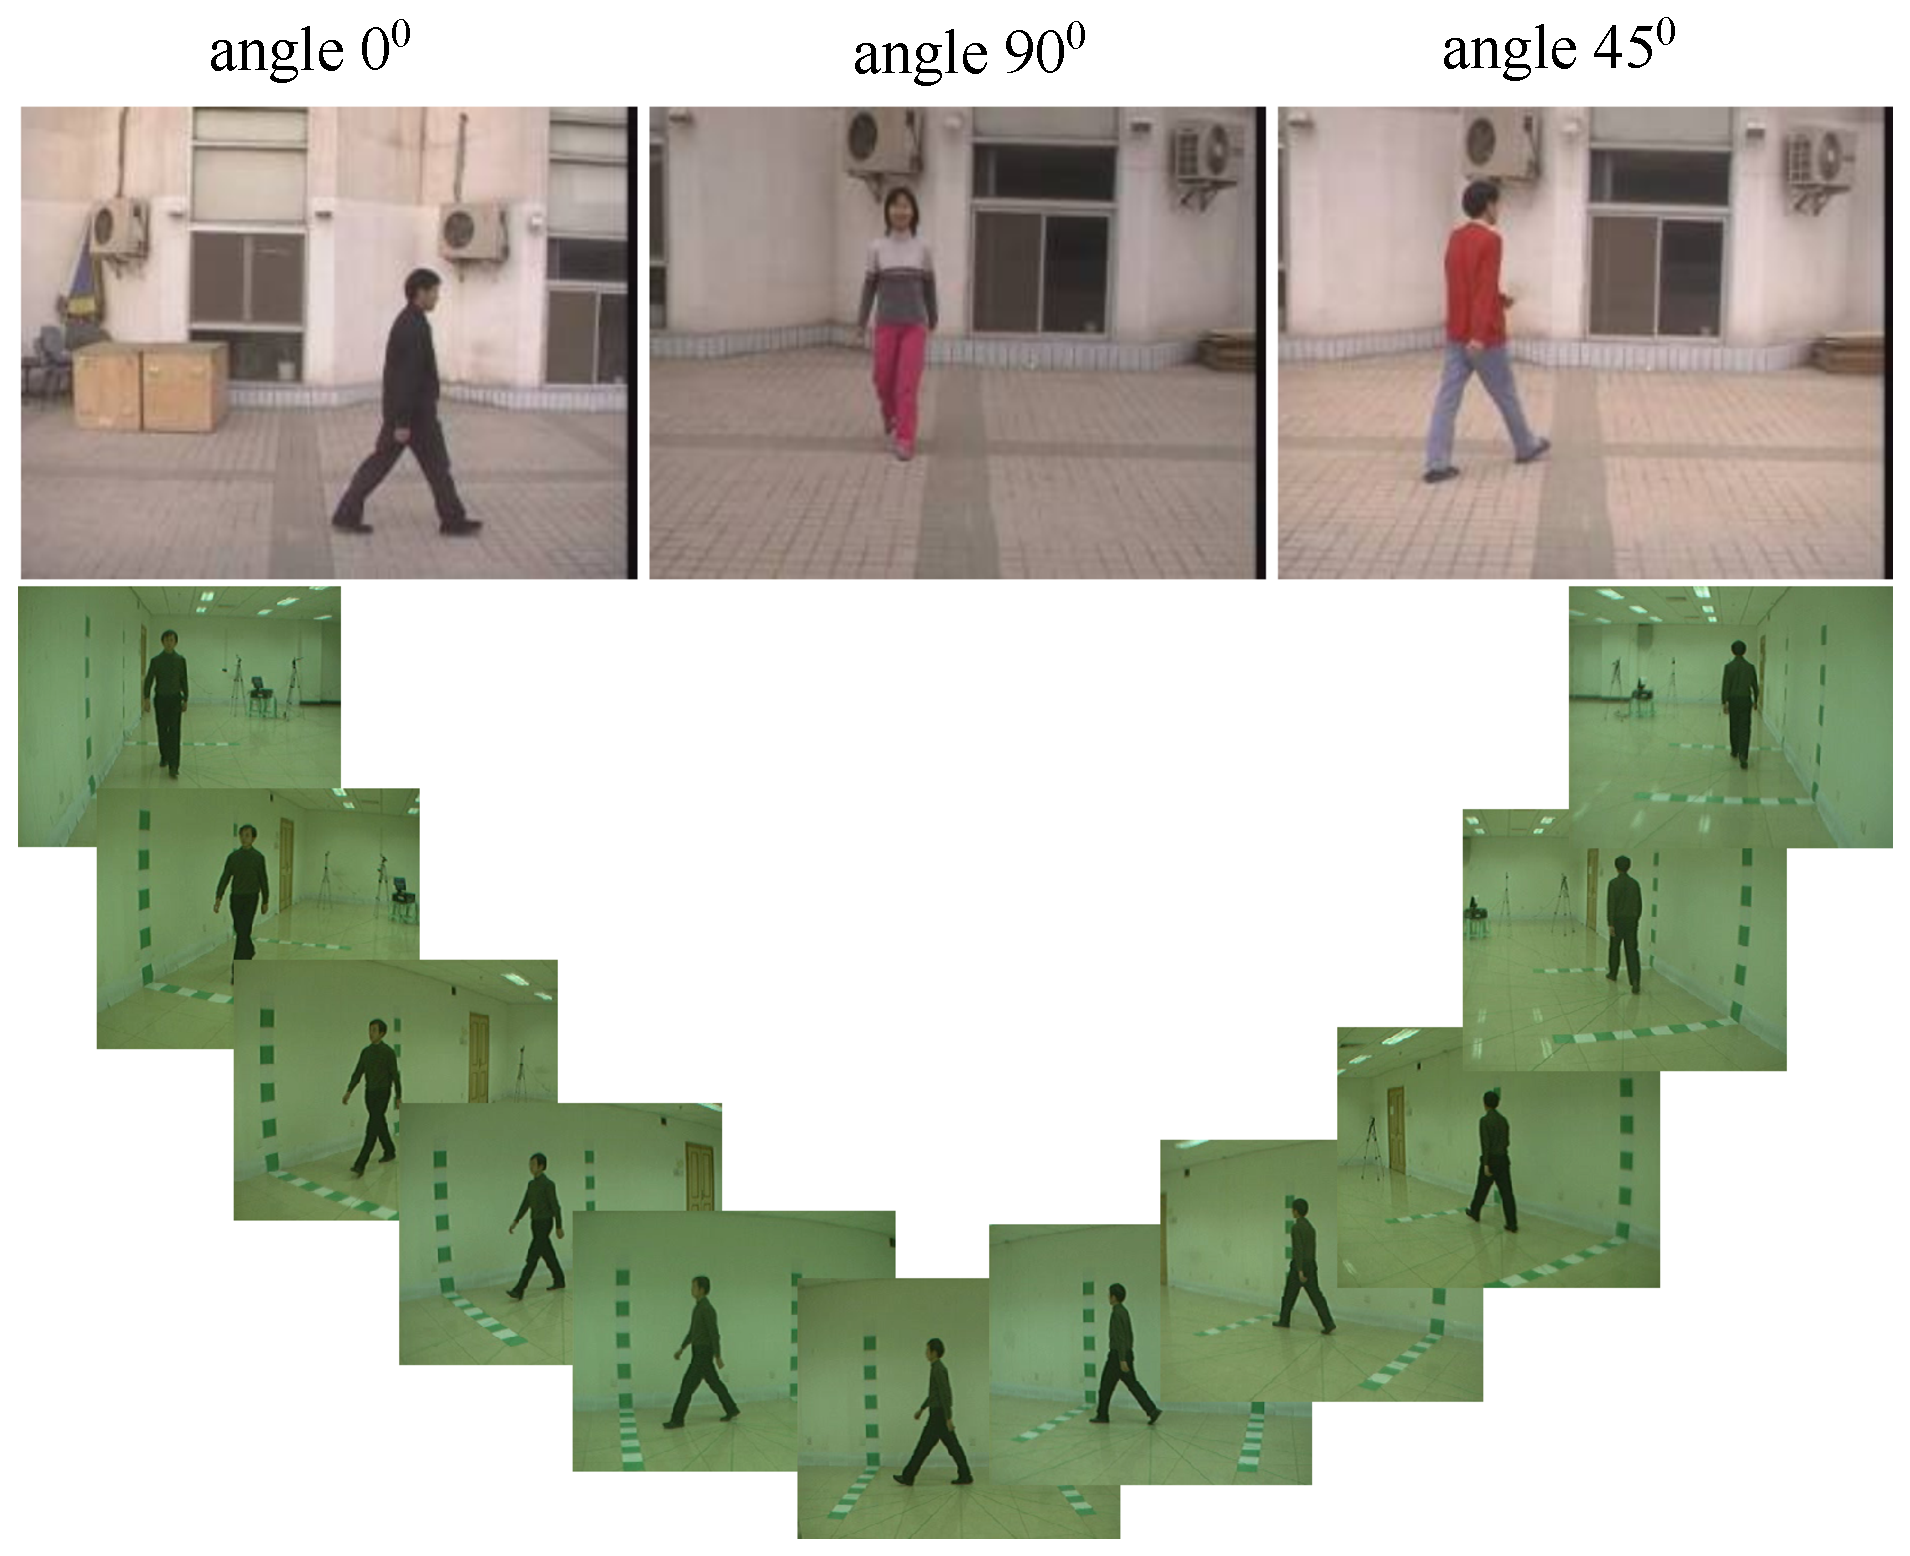
\includegraphics[width = 0.7\textwidth]{figures/casia_dataset.eps}
	\caption [Sample video frames of CASIA A and CASIA B dataset]
	{Sample video frames of CASIA A and CASIA B dataset. In top, some of the sample images from CASIA A dataset are shown where the subjects are walking along straight line in $ 3 $ different view angle, and in bottom, CASIA B dataset is shown with its $ 11 $ view angle.
	}
	\label{fig:casia_dataset}
\end{figure}


%-------------------------------------------------------------------------
\section{Single-View Gait Recognition}
\subsection{Experimental Evaluation on CASIA-A dataset}
Since, CASIA A dataset contains only $ 20 $ subjects each of which have only four gait sequence in three different angles, we trained three model for each of the gait angle with $ 20 $ output neurons in the final softmax layer of our proposed temporal network. To evaluate the performance of our proposed method on CASIA A dataset, we used leave-one-out cross validation rule, i.e., one sequence was set for testing and the remainder was set for training the network for each view angle. We compare our results with four other prevailing state-of-the-art gait recognition methods including Wang~\cite{Wang_03}, Goffredo~\cite{Goffredo_08}, Liu~\cite{Liu_16}, Lima~\cite{Lima_19}, Kusakunniran~\cite{Kusakunniran_09} (see Figure~\ref{fig:casia_a_result}). Table~\ref{table:casia_a_result} illustrates that the proposed method have achieved higher average correct class recognition rates (\gls{ccr}) $100.0\%$ compared to other methods.


\begin{table}
	\centering
	\caption [Comparison among different state-of-the-art gait recognition methods without view variation in all three view angles of CASIA A dataset]
	{Comparison among different state-of-the-art gait recognition methods without view variation in all three view angles of CASIA A dataset. It has been observed that the proposed method achieves higher average recognition rates \textbf{100.0\%} and outperforms other state-of-the-art methods by a large margin. \label{table:casia_a_result}}
	{\begin{tabular*}{30pc}{@{\extracolsep{\fill}}ccccc}\hline
			
			Methods &${0^{\circ}}$ &${45^{\circ}}$   &${90^{\circ}}$  &Mean\\
			\hline
			
			Wang~\cite{Wang_03} &88.75 &87.50 &90.00 &88.75\\
			
			\noalign{\smallskip}
			Goffredo~\cite{Goffredo_08} &100.0 &97.50 &91.00 &96.16\\ 
			
			\noalign{\smallskip}
			Liu~\cite{Liu_16} &85.00 &87.50 &95.00 &89.17\\ 
			
			\noalign{\smallskip}
			Lima~\cite{Lima_19} &92.50 &97.50 &98.75 &96.25 \\
			
			\noalign{\smallskip}
			Kusakunniran~\cite{Kusakunniran_09} &100  &100  &98.75 &99.58 \\
			
			\noalign{\smallskip}
			Proposed &{\textbf{100.0}} & {\textbf{100.0}} &{\textbf{100.0}} & {\textbf{100.0}}\\
			\hline
	\end{tabular*}}{}
\end{table}

\begin{figure}
	\centering
	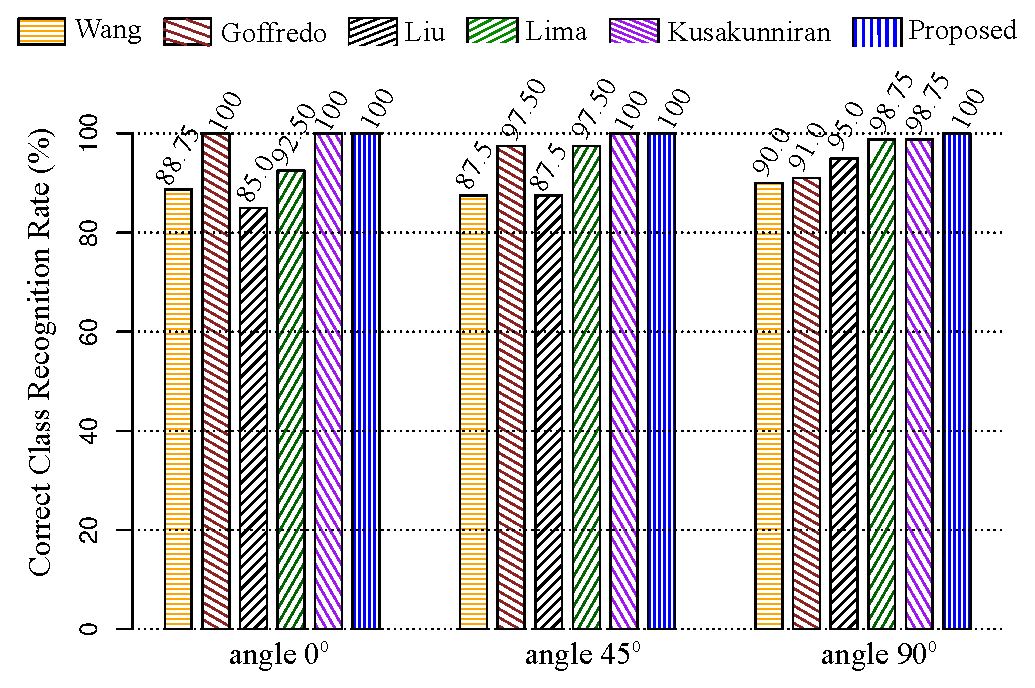
\includegraphics[width = 0.8\textwidth]{figures/casia_a_result.eps}
	\caption [Comparison in CCR at different view angles among proposed method with other prevailing gait recognition methods proposed in literature on CASIA A dataset]
	{Comparison in \gls{ccr} at different view angles among proposed method with other prevailing gait recognition methods proposed in literature on CASIA A dataset. Our method achieves $ \textbf{100\% }$ class recognition rate on all of the view angles which proved the efficacy of the proposed method. \label{fig:casia_a_result}
	}
	
\end{figure}



\subsection{Experimental Evaluation on CASIA-B Dataset}
\subsubsection{Experimental Setup}
We designed two experimental setups (A, B) in CASIA B dataset for evaluation. Experiment setup A was for evaluating the performance of the proposed method in single-view gait recognition. To investigate the robustness of view variation, comparison results of the proposed approach against other state-of-the-art methods in different view variations have been reported. Experiment setup B was designed for evaluating the cross-view recognition performance. 

For setup A, as demonstrated in Table~\ref{table:caisab_setup}, we divided the dataset into two groups where the first group which consists of 62 subjects was used to train the network. The second group contains rest of the subjects for evaluating the performance of the model. For setup B, the ratio between train and evaluation set was 24 to 100. In the evaluation set for both setup, 4 normal walking sequences of each subject are put into gallery set and rest 6 walking sequences consist three probe set (\textit{ProbeNM}, \textit{ProbeBG}, \textit{ProbeCL}). \textit{ProbeNM} consists of 2 other normal walking sequences where \textit{ProbeBG} and \textit{ProbeCL} consists of two subjects carrying bag and wearing coat respectively.


We divide CASIA-B dataset into two group where first group consists of 24 subjects and is used to train the network. The second group contains rest 100 subjects that are used to evaluate the performance of the model. In evaluation set, 4 normal walking sequences of each subject are put into gallery set and rest 6 walking sequences consist three probe set (\textit{ProbeNM}, \textit{ProbeBG}, \textit{ProbeCL}). \textit{ProbeNM} consists of 2 other normal walking sequences where 2 subjects carrying bag are kept in \textit{ProbeBG} and remaining 2 subjects wearing coat are kept in \textit{ProbeCL}. Table~\ref{table:caisab_setup} shows this experimental setup. 

\begin{table}[t]
	\centering
	\caption[Experimental setup for the CASIA B dataset]
	{Experimental setup for the CASIA B dataset. The dataset was divided into two different setups to organize two different types of experiment. the evaluation is subdivided into a gallery set and a probe set. Gallery set consists of the first 4 normal walking sequences of each subject and the probe set contains rest of the walking sequences  \label{table:caisab_setup}}
	
	{\begin{tabular*}{\textwidth}{cccccccc}\hline \noalign{\smallskip}
		\multirow{2}{*}{\textbf{Setup}} &\multicolumn{2}{c}{\textbf{Training set}} &\multicolumn{2}{c}{\textbf{Evaluation set}} & \multicolumn{2}{c}{\textbf{Sequences}}\\ \cline{2-7} \noalign{\smallskip}

		&ID &Total &ID &Total &Gallery &Probe\\ \hline \noalign{\smallskip}
		
		A &01 - 62 &62 &63 - 124 &62 &\multirow{2}{*}{${nm01 - nm04}$} &\multirow{2}{*}{
						\begin{tabular}{c}
						${nm05 - nm06}$\\ \hline
						${bg01 - bg02}$\\ \hline
						${cl01 - cl02}$\\
						\end{tabular}
		}\\[1.2ex] \cline{1 - 5} \noalign{\smallskip}
		B &01 - 74 &74 &75 - 124 &50 \\[1.2ex] \hline
	\end{tabular*}}{}
\end{table}


\subsubsection{Results on Single-View Gait Recognition of CASIA B Dataset without View Variation}
Experimental results of single-view gait recognition on all the three probe set of CASIA B dataset without view variation is illustrated in Table~\ref{table:resutl_without_view}. We achieved higher average recognition rate $ \textbf{97.80\%} $ and $\textbf{82.82\%} $ on the probe set of (\textit{ProbeBG}) and (\textit{ProbeCL}) respectively. This performance proves the robustness of our proposed method towards both carrying and clothing covariate conditions. We also achieved higher average class recognition rate $\textbf{99.41\%}$ on normal walking condition.

\begin{table}[t]
	\centering
	\caption [Correct class recognition rate (CCR) of proposed method in all three probe sets of CASIA B dataset]
	{Correct class recognition rate (\gls{ccr}) of proposed method in all three probe sets of CASIA B dataset. Here, column represents a specific view of gallery and probe set. It has been observed that the probe set of normal walking (\textit{ProbeNM}) achieves $ \textbf{99.41\%}$ average recognition rate while the ProbeBG and ProbeCL set achieve $ \textbf{97.80\%}$ and $\textbf{82.82\%}$ average recognition rates respectively. \label{table:resutl_without_view}}
	
	{\begin{tabular*}{22pc}{cccc}\hline
	Gallery Angle  &\textit{ProbeNM}  &\textit{ProbeBG} &\textit{ProbeCL} \\\hline\noalign{\smallskip} 
	${0^{\circ}}$	&100.0  &100.0  &81.52  \\\noalign{\smallskip}
	${18^{\circ}}$  &100.0  &100.0  &82.11  \\\noalign{\smallskip}
	${36^{\circ}}$	&100.0  &100.0  &83.58  \\\noalign{\smallskip}
	${54^{\circ}}$	&100.0  &100.0  &85.48  \\\noalign{\smallskip}
	${72^{\circ}}$	&100.0  &98.39 &84.46   \\\noalign{\smallskip}
	${90^{\circ}}$	&98.39  &96.77  &83.72  \\\noalign{\smallskip} 
	${108^{\circ}}$ &100.0  &96.77  &83.28  \\\noalign{\smallskip}
	${126^{\circ}}$ &100.0  &98.39  &84.16  \\\noalign{\smallskip}
	${144^{\circ}}$ &100.0  &98.39  &83.58  \\\noalign{\smallskip}
	${162^{\circ}}$	&98.39  &95.16  &80.65 \\\noalign{\smallskip}
	${180^{\circ}}$ &96.77  &91.93  &78.45  \\\noalign{\smallskip}
	Mean &\textbf{99.41}  &\textbf{97.80}  &\textbf{82.82} \\\hline
	\end{tabular*}}{}
\end{table}



\subsubsection{Comparison on Single-View Gait Recognition of CASIA B Dataset with State-of-the-art Methods without View Variation}
We compare our experimental results with other state-of-the-art methods such as GaitGANv2~\cite{Yu_19}, PTSN~\cite{Liao_17}, PoseGait~\cite{Liao_19}, Yu \textit{et al.}~\cite{Yu_17_spae} as shown in Figure~\ref{fig:comp_casia_b_without_view}. The experimental setup for all these methods were set A (see Table~\ref{table:caisab_setup}). Table~\ref{table:comp_casia_b_without_view} reports that CCR of the proposed method outperforms all other methods in all three covariate conditions of CASIA-B dataset; our method achieved average CCR of \textbf{93.34\%} with improvement of approx. \textbf{10\%} from PTSN.


\begin{table}[t]
	\centering
	\caption [Comparison between the proposed method and other state-of-the-art gait recognition methods in CASIA B dataset without view variation]
	{Comparison between the proposed method and other state-of-the-art gait recognition methods in CASIA B dataset without view variation. It has been observed that the proposed method outperforms other methods in all three probe set of CASIA B dataset. As the proposed method doesn't depend on any body point higher than knee, it shows the robustness towards these covariate factors. It also achieves higher average \gls{ccr} $\textbf{93.34\%}$ by outperforming other methods at a significant margin. \label{table:comp_casia_b_without_view}}
	
	{\begin{tabular*}{25pc}{ccccc}\hline
			
			Methods &\textit{ProbeNM} &\textit{ProbeBG} &\textit{ProbeCL} &Average\\
			\hline
			
			Liao \textit{et al.}~\cite{Liao_19} &96.92 &85.78 &68.11 &83.60 \\ 
			
			\noalign{\smallskip}
			Yu \textit{et al.}~\cite{Yu_17_spae}  &97.58  &72.14 &45.45 &71.72 \\
			
			\noalign{\smallskip}
			Yu \textit{et al.}~\cite{Yu_19} &98.24  &76.25  &42.89  &72.46 \\
			
			\noalign{\smallskip}
			Liao \textit{et al.}~\cite{Liao_19}  &96.63  &71.26  &54.18  &74.02 \\
			
			\noalign{\smallskip}
			Proposed &\textbf{99.41} &\textbf{97.80} &\textbf{82.82} &\textbf{93.34} \\
			\hline
	\end{tabular*}}{}
\end{table}

\begin{figure}
	\centering
	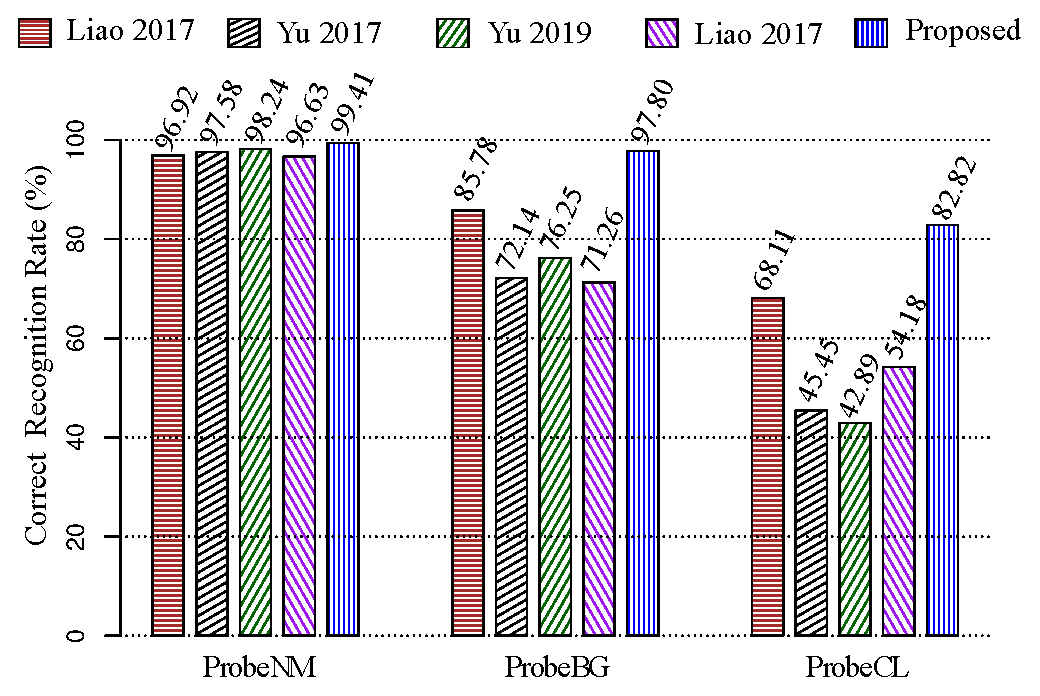
\includegraphics[width = 0.8\textwidth]{figures/comp_casia_b_without_view.eps}
	\caption [Correct class recognition rates (\%) of the proposed method with other state-of-the-art methods on all three probe set of CASIA-B dataset without view variation] 
	{Correct class recognition rates (\%) of the proposed method with other state-of-the-art methods on all three probe set of CASIA-B dataset without view variation. Proposed method demonstrates better performance compared to other by achieving $89.64\%$ and $96.45\%$ in two covariate conditions of CASIA-B dataset \textit{ProbeCL}, and \textit{ProbeBG} respectively. The result proves the robustness of proposed pose-based temporal network against carrying and clothing conditions variations.  \label{fig:comp_casia_b_without_view}
	}
\end{figure}


\subsubsection{Results on Single-View Gait Recognition of CASIA B Dataset with View Variation}
The performance of the proposed method on single-view gait recognition with view variation is demonstrated on Table~\ref{table:result_casia_b_with_view}. Here, for a specific gallery ($ \theta_g $) angle the average CCR (\%) of all eleven probe angles has been reported; our method achieved average CCR of $62.69\%$, $47.23\%$, and $33.46\%$ for Probe NM, probe BG, and probe CL respectively.


\begin{table}[t]
	\centering
	\caption{The average recognition rates for all three probe sets of CASIA B dataset. Each row represents the average value of all eleven probe angles at a specific gallery angle ($ \theta_g $) in all three probe sets. \label{table:result_casia_b_with_view}}
	{\begin{tabular*}{22pc}{cccc}\hline
			Gallery Angle &\textit{ProbeNM} &\textit{ProbeBG} &\textit{ProbeCL} \\\hline\noalign{\smallskip}
			${0^{\circ}}$	&61.73  &45.01  &32.40 \\\noalign{\smallskip}
			${18^{\circ}}$  &63.64  &47.80  &32.99 \\\noalign{\smallskip}
			${36^{\circ}}$	&67.30  &48.97  &34.46 \\\noalign{\smallskip}
			${54^{\circ}}$	&68.33  &50.15  &37.24 \\\noalign{\smallskip}
			${72^{\circ}}$	&68.33  &50.44  &39.0  \\\noalign{\smallskip}
			${90^{\circ}}$	&66.42  &49.12  &36.36  \\\noalign{\smallskip}
			${108^{\circ}}$ &64.22  &48.39  &34.75  \\\noalign{\smallskip}
			${126^{\circ}}$ &62.02  &47.07  &32.40  \\\noalign{\smallskip}
			${144^{\circ}}$ &58.80  &47.51  &31.82  \\\noalign{\smallskip}
			${162^{\circ}}$	&56.45  &44.13  &29.77  \\\noalign{\smallskip}
			${180^{\circ}}$ &52.35  &40.91  &26.83  \\\noalign{\smallskip}
			Mean &\textbf{62.69}  &\textbf{47.23} &\textbf{33.46} \\\hline
			
	\end{tabular*}}{}
\end{table}



\subsubsection{Comparison on Single-View Gait Recognition of CASIA B Dataset with State-of-the-art Methods with View Variation}
To better illustrate the robustness of our gait recognition method to view variation, the proposed method has been compared to three other state-of-the-art methods such as GaitGANv2~\cite{Yu_19}, PoseGait~\cite{Liao_19}, Yu \textit{et al.}~\cite{Yu_17_spae}.  It is observed from Figure~\ref{fig:comp_casia_b_with_view} and Table~\ref{table:comp_casia_b_with_view} comparison that proposed method outperforms other in covariate variation and achieves comparable performance in normal walking. 

Since, to recognize gait, we consider features based on effective body joints, hence our method doesn't get affected by the variation in covariate conditions compared to other appearance-based method or other model-based methods which consider ineffective features to build their gait descriptor. That’s why our method is proven to be less sensitive to view angle variation and performs better in carrying-bag and clothing condition. 

\begin{table}
	\centering
	\caption [Comparison among different state-of-the-art methods for gait recognition with view variation in all three probe sets of CASIA B dataset]
	{Comparison among different state-of-the-art methods for gait recognition with view variation in all three probe sets of CASIA B dataset. Each row represents the average value of all the gallery view's average recognition rate. It has been seen that, similar to first experiment, the proposed method achieves higher performance in two different probe set (\textit{ProbeBG}, \textit{ProbeCL}) and comparable performance in normal walking with to other prevailing methods. \label{table:comp_casia_b_with_view}}
		
	{\begin{tabular*}{22pc}{cccc}\hline
				
				Methods &\textit{ProbeNM} &\textit{ProbeBG} &\textit{ProbeCL}\\
				\hline
				
				\noalign{\smallskip}
				Yu \textit{et al.}~\cite{Yu_17_spae} &62.82 &40.38 &26.05 \\ 
				
				
				\noalign{\smallskip}
				Yu \textit{et al.}~\cite{Yu_19} &66.34  &46.17  &25.91  \\
				
				\noalign{\smallskip}
				Liao \textit{et al.}~\cite{Liao_19}  &63.78  &42.52  &31.98  \\
				
				\noalign{\smallskip}
				Proposed &\textbf{62.69} &\textbf{47.23} &\textbf{33.46}\\
				\hline
\end{tabular*}}{}
\end{table}

\begin{figure}
	\centering
	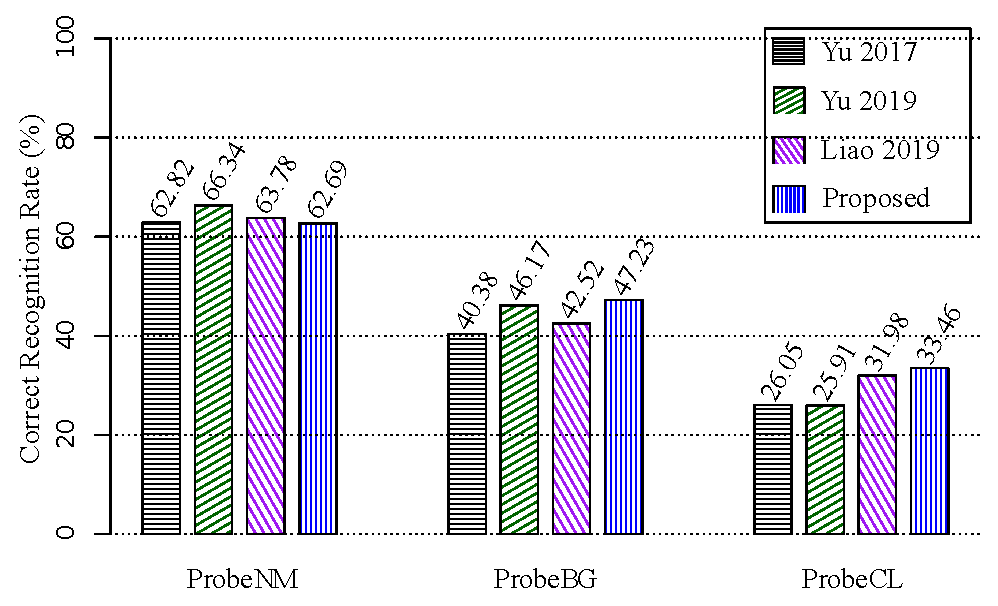
\includegraphics[width = 0.8\textwidth]{figures/comp_casia_b_with_view.eps}
	\caption [Comparison with different state-of-the-art methods for gait recognition with view variation in all three probe set of CASIA B dataset]
	{Comparison with different state-of-the-art methods for gait recognition with view variation in all three probe set of CASIA B dataset. Here, the value reported for each algorithm is the average of all the gallery view's average \gls{ccr}. Proposed method outperforms other state-of-the-art methods achieving $47.23\%$ and $33.46\%$ in two covariate conditions \textit{ProbeBG}, and \textit{ProbeCL} respectively.   \label{fig:comp_casia_b_with_view}
	}
	
\end{figure}




%---------------------------------------------------------------------------------------------- 
\section{Cross-View Gait Recognition}
The gait recognition scheme in which gallery and probe set are getting matched from two different views is commonly known as cross-view gait recognition.

\subsection{Comparison with the State-of-the-art Methods of CASIA B Dataset on Cross-View Gait Recognition}
To show the effectiveness of our method in cross-view recognition, we make the comparison between the proposed method and three other state-of-the-art methods including CNN~\cite{Wu_17}, CMCC~\cite{Kusakunniran_14}, and GEI-SVR~\cite{Kusakunniran_10} with the same experimental setup. The probe angles were selected $0^{\circ}, 54^{\circ}, 90^{\circ}$, and $126^{\circ}$ for comparison. 

Although, the proposed method contains only one model to handle any view angle variation, it achieves comparable performance with other prevailing state-of-the-art methods proposed in literature which were specially designed and trained for cross-view gait recognition. From Table~\cite{table:comp_casia_b_cross_view}, it is seen that CNN~\cite{Wu_17} achieves the highest recognition rates when the view variation is large due to the use of supervised information of all gallery angles during training.


\begin{table}
	\centering
	\caption[Comparison of our proposed method with the previous best results of cross-view gait recognition ]
	{Comparison of our proposed method with the previous best results of cross-view gait recognition at different probe angles of CASIA B dataset by \gls{ccr}(\%). The network was trained according to experimental setup B to have the same setup with other methods. \label{table:comp_casia_b_cross_view}}
	
	{\begin{tabular*}{29pc}{c|c|cccc}\hline  \rule{0pt}{2ex}
	Probe View &Gallery View &CNN &CMCC &GEI-SVR  &\textbf{Proposed} \\ \hline\rule{0pt}{3ex}
	
	% first gallery angle
	\multirow{2}{*}{$0^{\circ}$} &$18^{\circ}$ &95.0 &85.0 &84.0 &\textbf{97.0} \\\rule{0pt}{2ex}
	
					&$36^{\circ}$ &73.5 &47.0 &45.0 &\textbf{80.0} \\ \hline\rule{0pt}{3ex}
	
	
	% second gallery angle
	\multirow{4}{*}{$54^{\circ}$} &$18^{\circ}$ &\textbf{91.5} &65.0 &64.0  &83.0 \\\rule{0pt}{2ex}
	
			&$36^{\circ}$ &98.5 &97.0 &95.0 &\textbf{100.0} \\\rule{0pt}{2ex}
	
			&$72^{\circ}$ &98.5 &95.0 &93.0 &\textbf{100.0} \\\rule{0pt}{2ex}
	
			&$90^{\circ}$ &\textbf{93.0} &63.0 &59.0 &83.0 \\\hline\rule{0pt}{3ex}
	
	
	% third gallery angle
	\multirow{4}{*}{$90^{\circ}$} &$54^{\circ}$ &-- &66.0 &63.0 &\textbf{84.0 }\\\rule{0pt}{2ex}
	
		&$72^{\circ}$ &\textbf{99.5} &96.0 &95.0 &96.0 \\ \rule{0pt}{2ex}
	
		&$108^{\circ}$ &\textbf{99.5} &95.0 &95.0 &95.0 \\ \rule{0pt}{2ex}
	
		&$126^{\circ}$ &-- &68.0 &65.0 &\textbf{71.0} \\\hline\rule{0pt}{3ex}
	
	
	% four gallery angle
	\multirow{4}{*}{$126^{\circ}$} &$90^{\circ}$ &\textbf{92.0} &78.0 &78.0 &76.0 \\\rule{0pt}{2ex}
			&$108^{\circ}$ &\textbf{99.0} &98.0 &98.0 &92.0 \\\rule{0pt}{2ex}
			&$144^{\circ}$ &97.0 &\textbf{98.0} &\textbf{98.0} &96.0 \\\rule{0pt}{2ex}
			&$162^{\circ}$ &\textbf{83.0} &75.0 &74.0 &77.0 \\\hline
	\end{tabular*}}{} 
\end{table}

The comparison in Table~\ref{table:comp_casia_b_cross_view} also illustrates that the proposed method performs better when the view variation is small. The reason for not achieving better performance at large view variation is because it was trained with only one viewing angle.  



%---------------------------------------------------------------------------------------------- 
\section{Multi-View Gait Recognition}
In multi-view gait recognition, multiple views of gallery gaits are combined to recognize probe set for an unknown gait view. In our work, for multi-view gait recognition, we trained a two-stage network in which we initially identify the walking direction of a gait video using a 3D-CNN network. 

\begin{table}
	\centering
	\caption [Comparison with other state-of-the-art methods on all three probe set of CASIA-B dataset in multi-view gait recognition]
	{Comparison with other state-of-the-art methods on all three probe set of CASIA-B dataset in multi-view gait recognition. From the comparison, it is been observed that proposed two-stage network achieves higher average recognition rates in 8 of 11 different probe angles.\label{table:comp_multi_view}}
	\setlength{\tabcolsep}{3.5pt}
	\small
	{\begin{tabular*}{\textwidth}{|c|c|cccc cccc ccc|} \cline{1-13}\rule{0pt}{3ex}
		% header
		&Methods &${0^{\circ}}$ &${18^{\circ}}$  &${36^{\circ}}$ &${54^{\circ}}$ &${72^{\circ}}$	&${90^{\circ}}$	&${108^{\circ}}$ &${126^{\circ}}$ &${144^{\circ}}$ &${162^{\circ}}$  &${180^{\circ}}$ \\\cline{1-13}\rule{0pt}{3ex}
					
		% first probe set
		\multirow{4}{*}{\rotatebox{90}{Normal}} &Dupuis &97.2 &99.6 &97.2 &96.3 &98.8 &98.4 &97.1 &97.6 &97.14 &93.0 &96.0 \\\rule{0pt}{3ex}
		
		&VI-MGR &100.0 &99.0 &100.0 &99.0 &100.0 &100.0 &99.0 &99.0 &100.0 &100.0 &99.0 \\ \rule{0pt}{3ex}
		
		&Isaac &98.5 &99.0 &99.0 &97.0 &97.5 &96.0 &95.0 &97.5 &94.0 &93.9 &99.0 \\\rule{0pt}{3ex}
		
		&\textbf{Proposed} &100.0  &100.0  &100.0  &100.0  &100.0  &98.4  &100.0  &100.0  &100.0  &98.4  &96.8 \\\cline{1-13}\rule{0pt}{3ex}
	
	
	
		% second probe set
		\multirow{4}{*}{\rotatebox{90}{Bag}} &Dupuis &73.2 &74.1 &74.7 &76.3 &78.5 &75.8 &76.3 &76.7 &73.4 &73.2 &74.6 \\\rule{0pt}{3ex} 

		&VI-MGR &93.0 &89.0 &89.0 &90.0 &77.0 &80.0 &82.0 &84.0 &92.0 &93.0 &89.0 \\\rule{0pt}{3ex}

		&Isaac &95.0 &98.5 &96.5 &96.0 &97.5 &93.5 &93.5 &94.0 &92.5 &91.3 &94.4 \\\rule{0pt}{3ex}

		&\textbf{Proposed}  &100 &100 &100 &100 &98.39 &96.77 &96.77 &98.39 &98.39 &95.16 &91.93 \\\hline\rule{0pt}{3ex}


		% third probe set
		\multirow{4}{*}{\rotatebox{90}{Coat}} &Dupuis &81.64 &87.39 &86.29 &84.34 &89.96 &91.86 &89.50 &85.04 &72.24 &78.40 &82.70\\\rule{0pt}{3ex}
		
		&VI-MGR &67.0 &56.0 &70.0 &80.0 &71.0 &75.0 &77.0 &75.0 &65.0 &64.0 &66.0 \\\rule{0pt}{3ex}
		
		&Isaac &97.0 &99.5 &97.5 &94.0 &88.0 &90.5 &89.5 &94.5 &92.0 &91.3 &94.0 \\\rule{0pt}{3ex}
		
		&\textbf{Proposed} &81.52 &82.11 &83.58 &85.48 &84.46 &83.72 &83.28 &84.16 &83.58 &80.65 &78.45 \\\cline{1-13}
\end{tabular*}}{} 
\end{table}


%------------------------------------------------------------------------- 
\subsection{Comparison with the State-of-the-art Methods on Multi-View Gait Recognition}
We tested the proposed 3D-CNN network with all three probe set of CASIA-B dataset and have achieved \textbf{100\%} identification accuracy in all viewpoint angles proving the fact that our 3D-CNN is efficient in classifying walking direction from gait videos. Table~\ref{table:result_wd_identification} illustrates our test result. 


\begin{table}[t]
	\centering
	\caption[Correct walking direction identification rate (\%) of proposed 3D-CNN network on all three probe set of CASIA-B dataset]
	{Correct walking direction identification rate (\%) of proposed 3D-CNN network on all three probe set of CASIA-B dataset. The network achieved \textbf{100\%} identification accuracy in all of the 11 view angles. \label{table:result_wd_identification}}
	
	{\begin{tabular*}{35pc}{cccc cccc cccc}\hline \noalign{\smallskip}
			View angle &${0^{\circ}}$	&${18^{\circ}}$  &${36^{\circ}}$ &${54^{\circ}}$	&${72^{\circ}}$	&${90^{\circ}}$	&${108^{\circ}}$ &${126^{\circ}}$ &${144^{\circ}}$ &${162^{\circ}}$  &${180^{\circ}}$ \\\hline \noalign{\smallskip}
			
			Rate(\%) &100 &100 &100 &100 &100 &100 &100 &100 &100 &100 &100 \\ \hline
	\end{tabular*}}{}
\end{table}

To evaluate the performance of the proposed two-stage network, we compare it with the recent state-of-the-art multi-view gait recognition methods such as Dupuis~\textit{et al.}~\cite{Dupuis_13}, Isaac~\textit{et al.}~\cite{Isaac_17}, and VI-MGR~\cite{Choudhury_15} on all three probe set of CASIA-B dataset. The comparison, as illustrated in Table~\ref{table:comp_multi_view} and Fig.~\ref{fig:comp_casia_b_multi_view}, shows that the proposed method exceeds the previous best in result all three probe set by a significant margin. It outperforms other in $ \textbf{8} $ of $ 11 $ total probe angles.

\begin{figure}
	\centering
	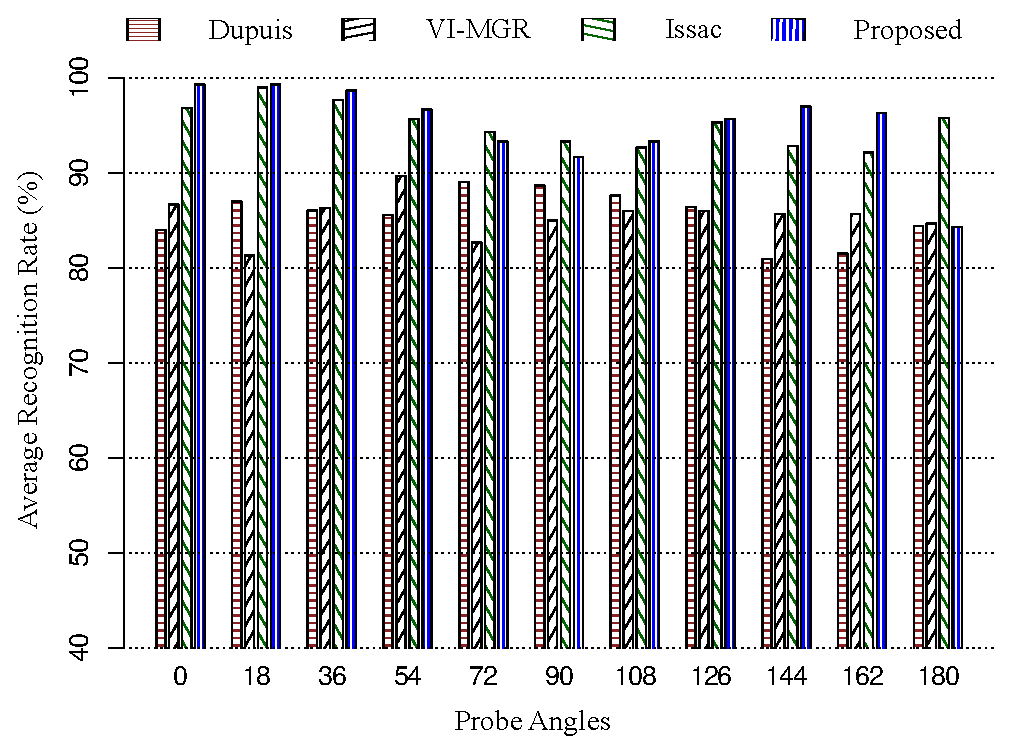
\includegraphics[width= 0.9\textwidth]{figures/comp_casia_b_multi_view.eps}
	\caption [Average recognition rates(\%) of the proposed method compared to the other state-of-the-art methods in 	multi-view gait recognition]{
		Average recognition rates(\%) of the proposed method compared to the other state-of-the-art methods in multi-view gait recognition. Proposed method achieves higher average recognition accuracy on 8 of total 11 probe angles of CASIA-B dataset compared other methods in literature. \label{fig:comp_casia_b_multi_view}
	}

\end{figure}

